Kontekst Finansowania to poddziedzina generyczna (\textit{Generic Subdomain}), która stanowi most komunikacyjny pomiędzy salonem samochodowym a rynkiem usług finansowych (banki, firmy leasingowe). Głównym wyzwaniem architektonicznym w tym obszarze jest zapewnienie niezawodnej komunikacji i translacji danych przy jednoczesnej ochronie jądra systemu przed zmieniającymi się standardami zewnętrznych interfejsów API.

\subsubsection{Kanwa Kontekstu Finansowania}
\begin{figure}[H]
    \centering
    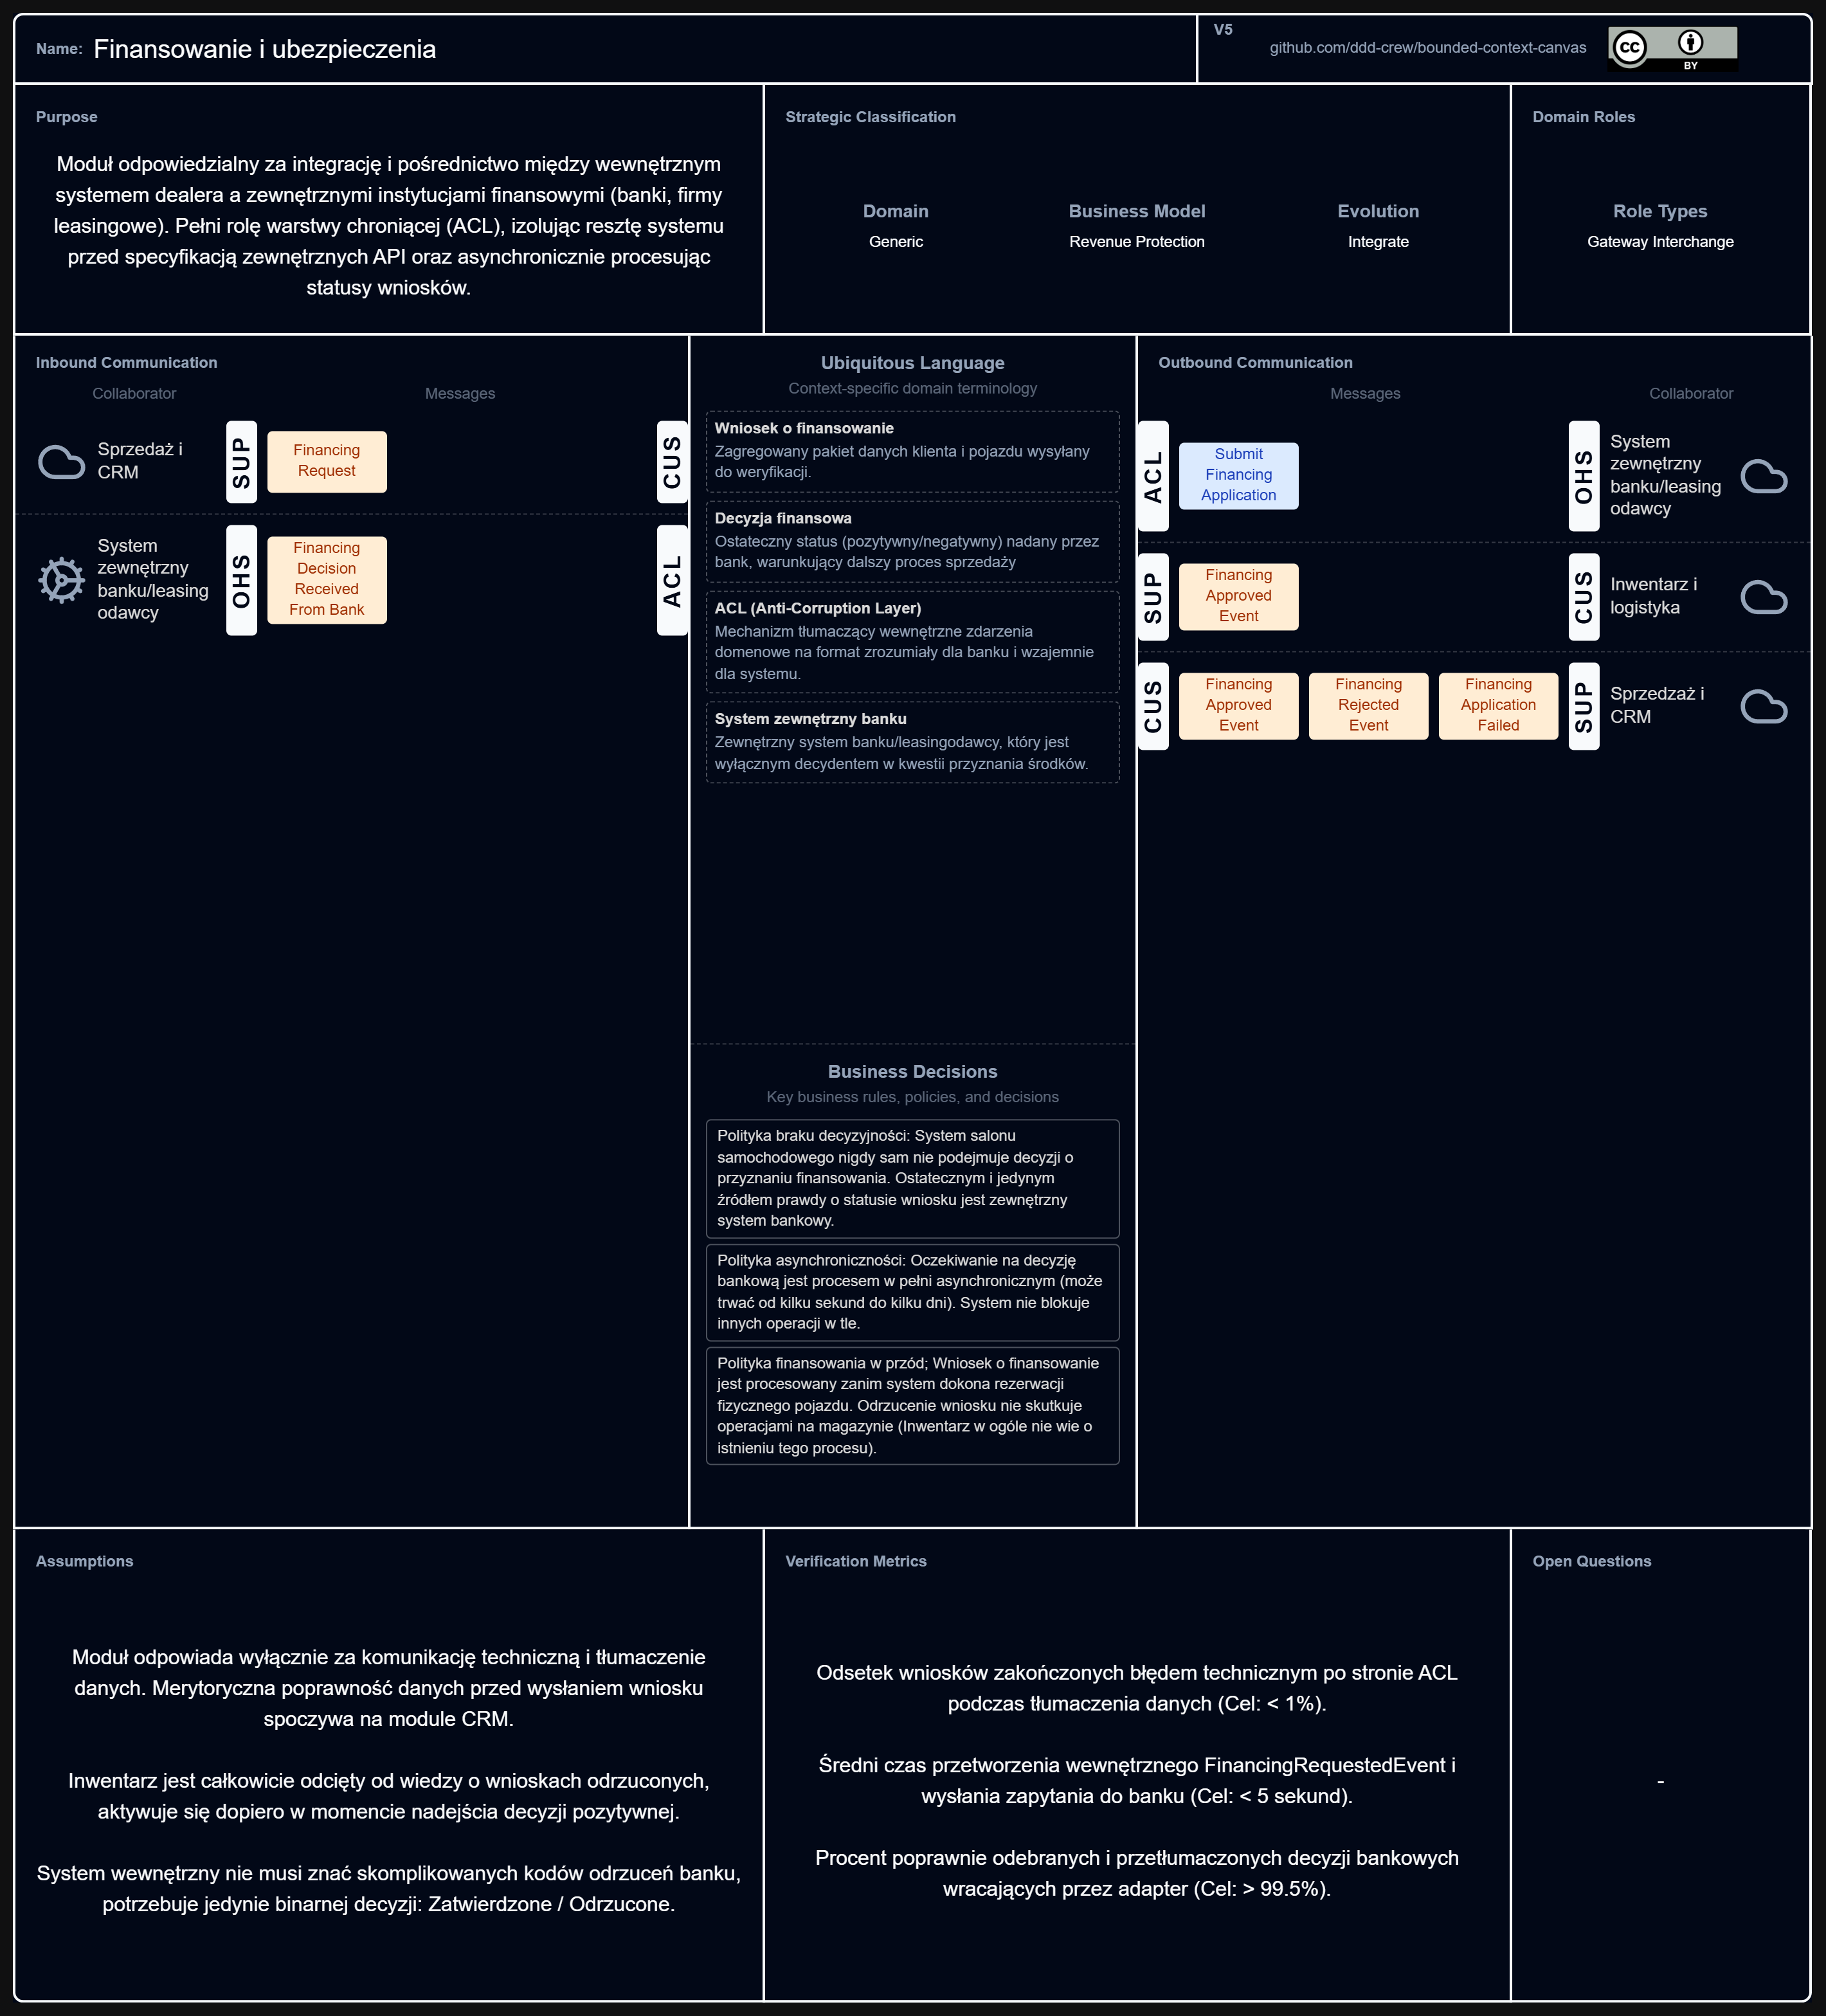
\includegraphics[width=\textwidth]{media/bounded-context-canvas/final/FIU_K6_TOTAL_FINAL.png}
    \caption{Kanwa Kontekstu Kontekstu Finansowania}
    \label{fig:hex_billing}
\end{figure}


\subsubsection{Przypadki użycia Kontekstu Finansowania}
% =====================================================
\textbf{UC-FIN-01: Złożenie wniosku o finansowanie}

\begin{longtable}{|p{4cm}|p{11cm}|}
\hline
\textbf{Element} & \textbf{Opis} \\
\hline

Identyfikator & UC-FIN-01 \\
\hline

Nazwa & Złożenie wniosku o finansowanie \\
\hline

Opis & 
Proces zebrania danych z zamówienia, ich translacji i wysłania zapytania o zdolność kredytową/leasingową klienta do systemu bankowego. \\
\hline

Aktor główny & System (Kontekst Finansowania) \\
\hline

Aktorzy pomocniczy & System zewnętrzny banku \\
\hline

Warunki wstępne & 
Kontekst otrzymał zdarzenie \textit{FinancingRequestedEvent} (Klient w CRM zdecydował się na leasing/kredyt i podał wymagane dane). \\
\hline

Warunki końcowe & 
Wniosek zostaje wysłany do systemu zewnętrznego banku, a system oczekuje na decyzję (status finansowania: Oczekujący). \\
\hline

Scenariusz główny & 
\begin{enumerate}
    \item Kontekst reaguje na zdarzenie \textit{FinancingRequestedEvent}.
    \item System agreguje dane pojazdu (cena, VIN/model) oraz dane klienta (NIP, dochody).
    \item System tłumaczy (poprzez ACL) dane na strukturę wymaganą przez API banku (np. dedykowany JSON/XML).
    \item System wysyła żądanie autoryzacji do systemu zewnętrznego banku.
    \item System oznacza wniosek lokalnie statusem "W trakcie weryfikacji bankowej".
\end{enumerate} \\
\hline

Scenariusze alternatywne & 
\begin{itemize}
    \item [A1] Błąd komunikacji z bankiem: API banku nie odpowiada, system zawiesza proces i ponawia próbę po określonym czasie.
    \item [A2] Odrzucenie walidacji po stronie banku: System banku natychmiast zwraca błąd o braku wymaganych danych (np. błędny NIP). System emituje zdarzenie \textit{FinancingApplicationFailed}, aby handlowiec poprawił wniosek wraz z Klientem.
\end{itemize} \\
\hline
\end{longtable}

\begin{figure}[H]
    \centering
    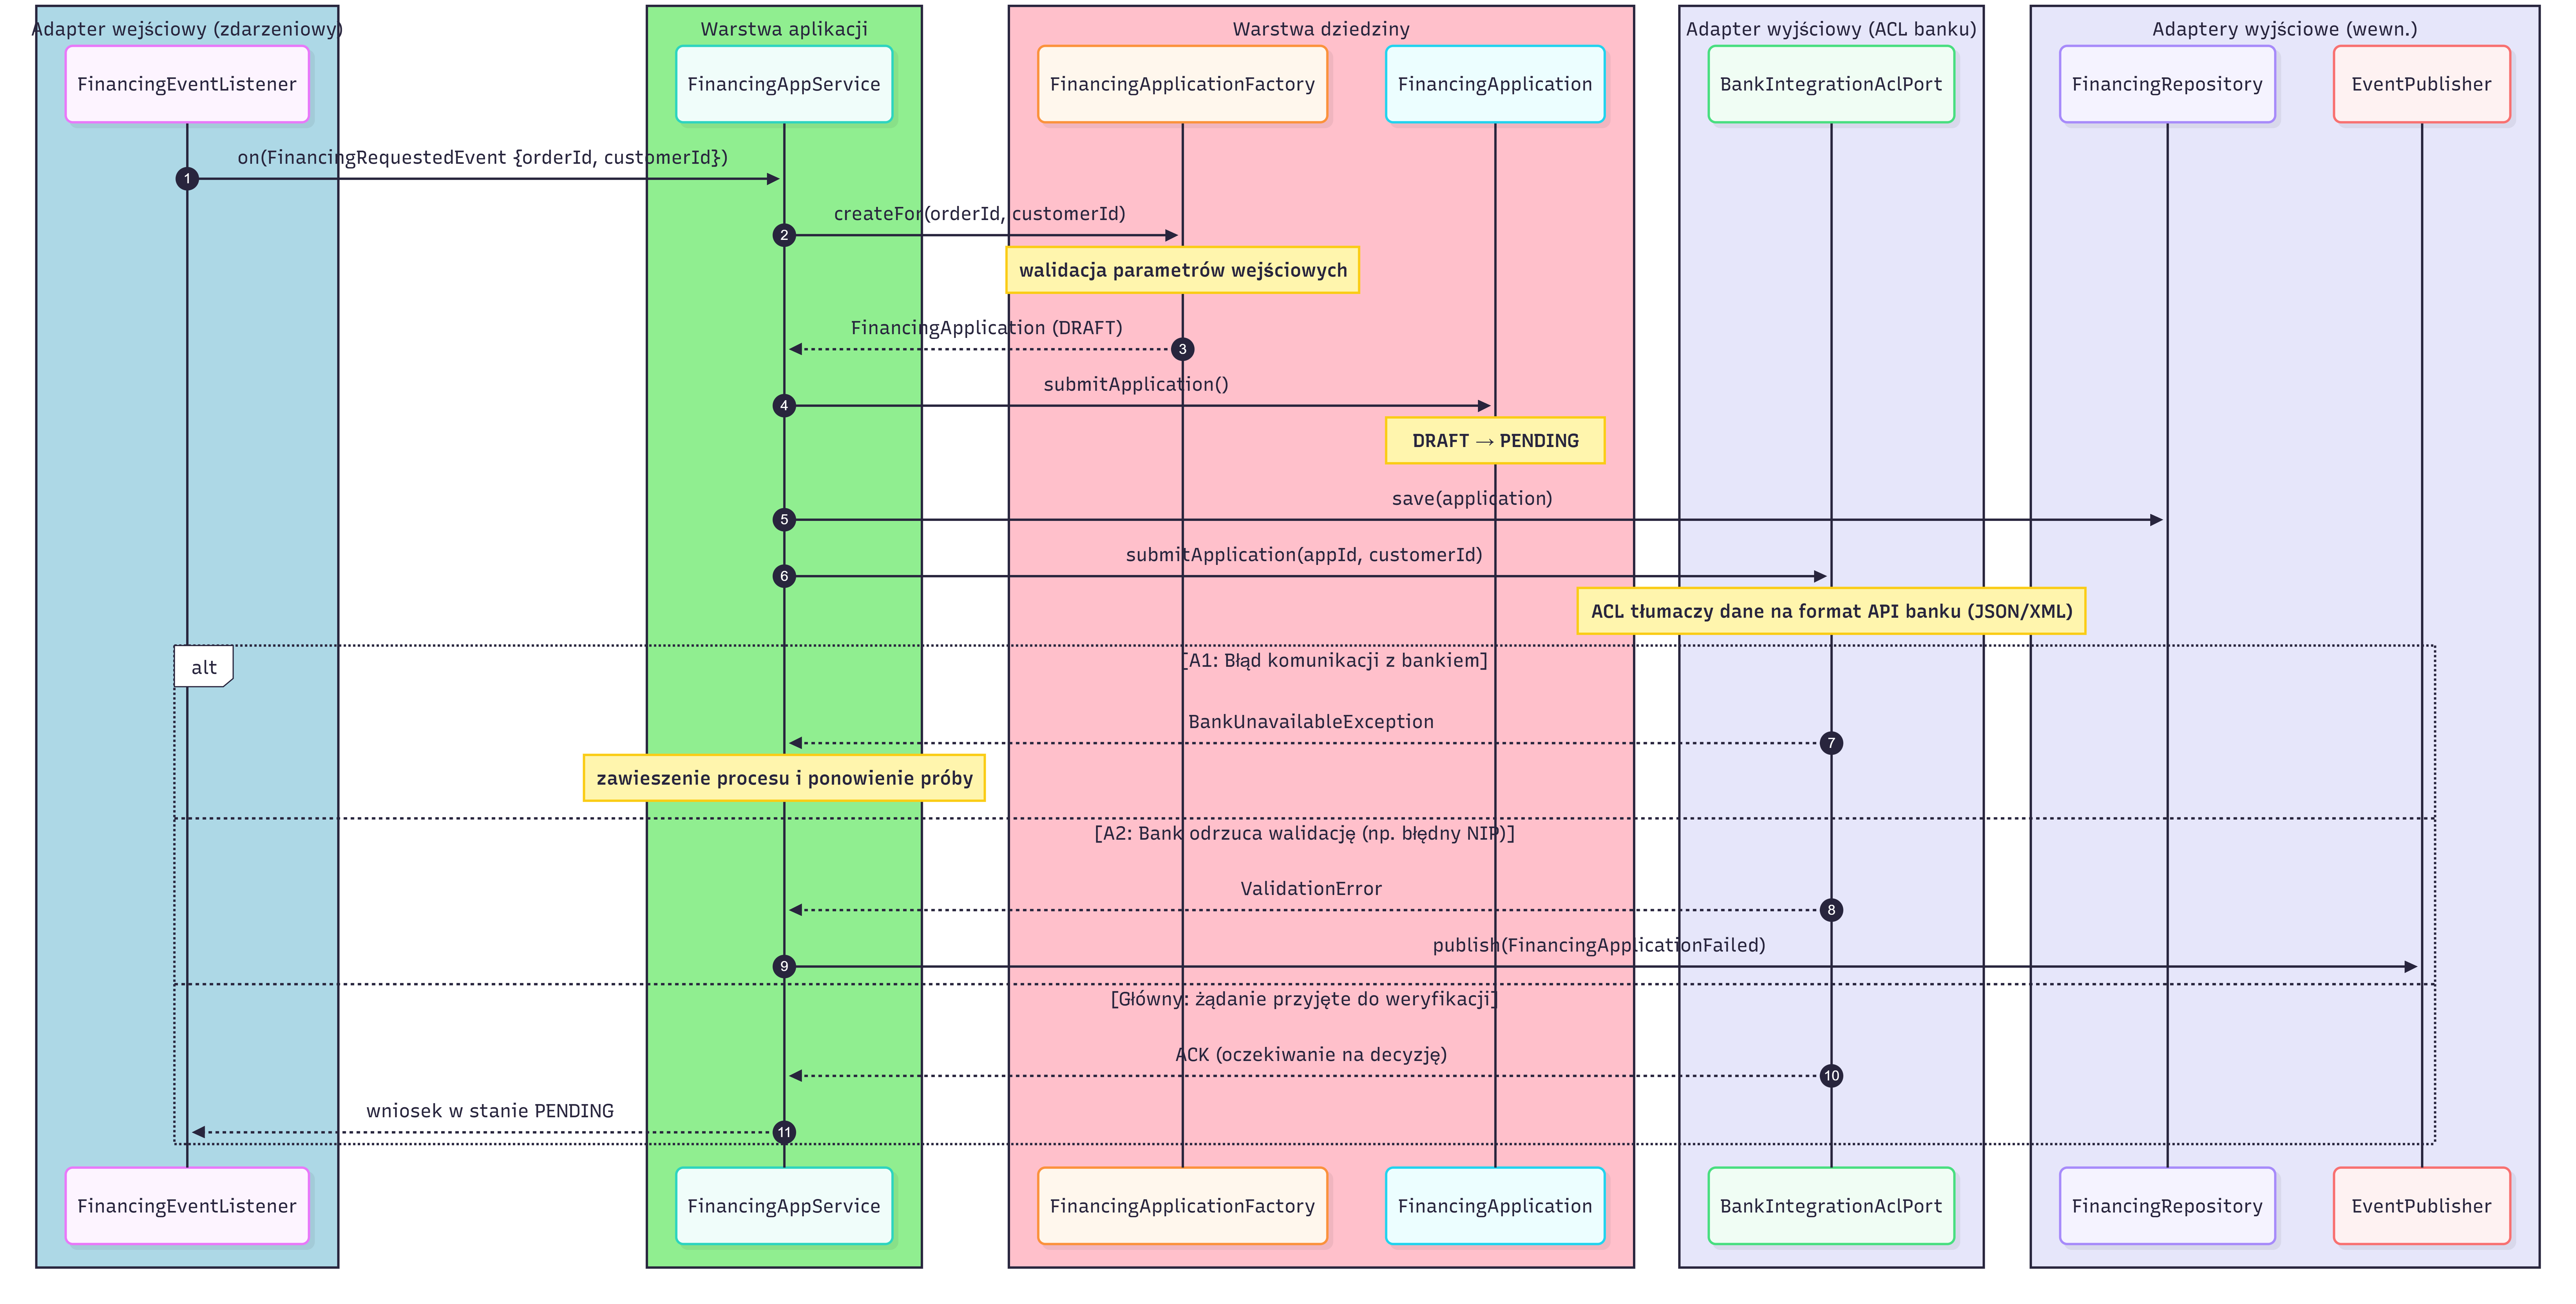
\includegraphics[width=1\textwidth]{media/diagramy_sekwencji/kontekst-finansowania/UC-FIN-01-Sekwencji.png}
    \caption{Diagram sekwencji dla przypadku użycia UC-FIN-01: Złożenie wniosku o finansowanie}
    \label{fig:seq_uc_fin_01}
\end{figure}

% =====================================================
\textbf{UC-FIN-02: Przetworzenie decyzji o finansowaniu}

\begin{longtable}{|p{4cm}|p{11cm}|}
\hline
\textbf{Element} & \textbf{Opis} \\
\hline

Identyfikator & UC-FIN-02 \\
\hline

Nazwa & Przetworzenie decyzji o finansowaniu \\
\hline

Opis & 
Odbiór i procesowanie asynchronicznej decyzji z banku oraz ogłoszenie jej wyniku wewnątrz systemu. \\
\hline

Aktor główny & System (Kontekst Finansowania i Ubezpieczeń) \\
\hline

Aktorzy pomocniczy & Adapter bankowy \\
\hline

Warunki wstępne & 
W systemie istnieje wniosek o finansowanie o statusie "W trakcie weryfikacji bankowej". Kontekst otrzymał zdarzenie z adaptera bankowego \textit{FinancingDecisionReceivedFromBank}. \\
\hline

Warunki końcowe & 
Decyzja zapisana w systemie, wyemitowane odpowiednie zdarzenie końcowe \textit{FinancingApprovedEvent} lub \textit{FinancingRejectedEvent}. \\
\hline

Scenariusz główny & 
\begin{enumerate}
    \item System reaguje na zdarzenie \textit{FinancingDecisionReceivedFromBank}.
    \item System bankowy przekazuje pozytywną decyzję o finansowaniu.
    \item System weryfikuje odpowiedź i aktualizuje status wniosku w lokalnej bazie.
    \item System emituje zdarzenie \textit{FinancingApprovedEvent}.
\end{enumerate} \\
\hline

Scenariusze alternatywne & 
\begin{itemize}
    \item [A1] Decyzja odmowna: W kroku 2 system zewnętrzny banku przekazuje decyzję negatywną. System (po weryfikacji) emituje zdarzenie \textit{FinancingRejectedEvent}.
\end{itemize} \\
\hline
\end{longtable}

\begin{figure}[H]
    \centering
    \includegraphics[width=1\textwidth]{media/diagramy_sekwencji/kontekst-finansowania/UC-FIN-02-Sekwencji.png}
    \caption{Diagram sekwencji dla przypadku użycia UC-FIN-02: Przetworzenie decyzji o finansowaniu}
    \label{fig:seq_uc_fin_02}
\end{figure}

\subsubsection{Architektura Kontekstu Finansowania i Wzorzec ACL}

Kontekst Finansowania został zaprojektowany w oparciu o architekturę heksagonalną. Diagram Architektury przedstawiono na rysunku \ref{fig:hex_finance}.

% MIEJSCE NA DIAGRAM ARCHITEKTURY (Finansowanie Flowchart)
\begin{figure}[H]
    \centering
    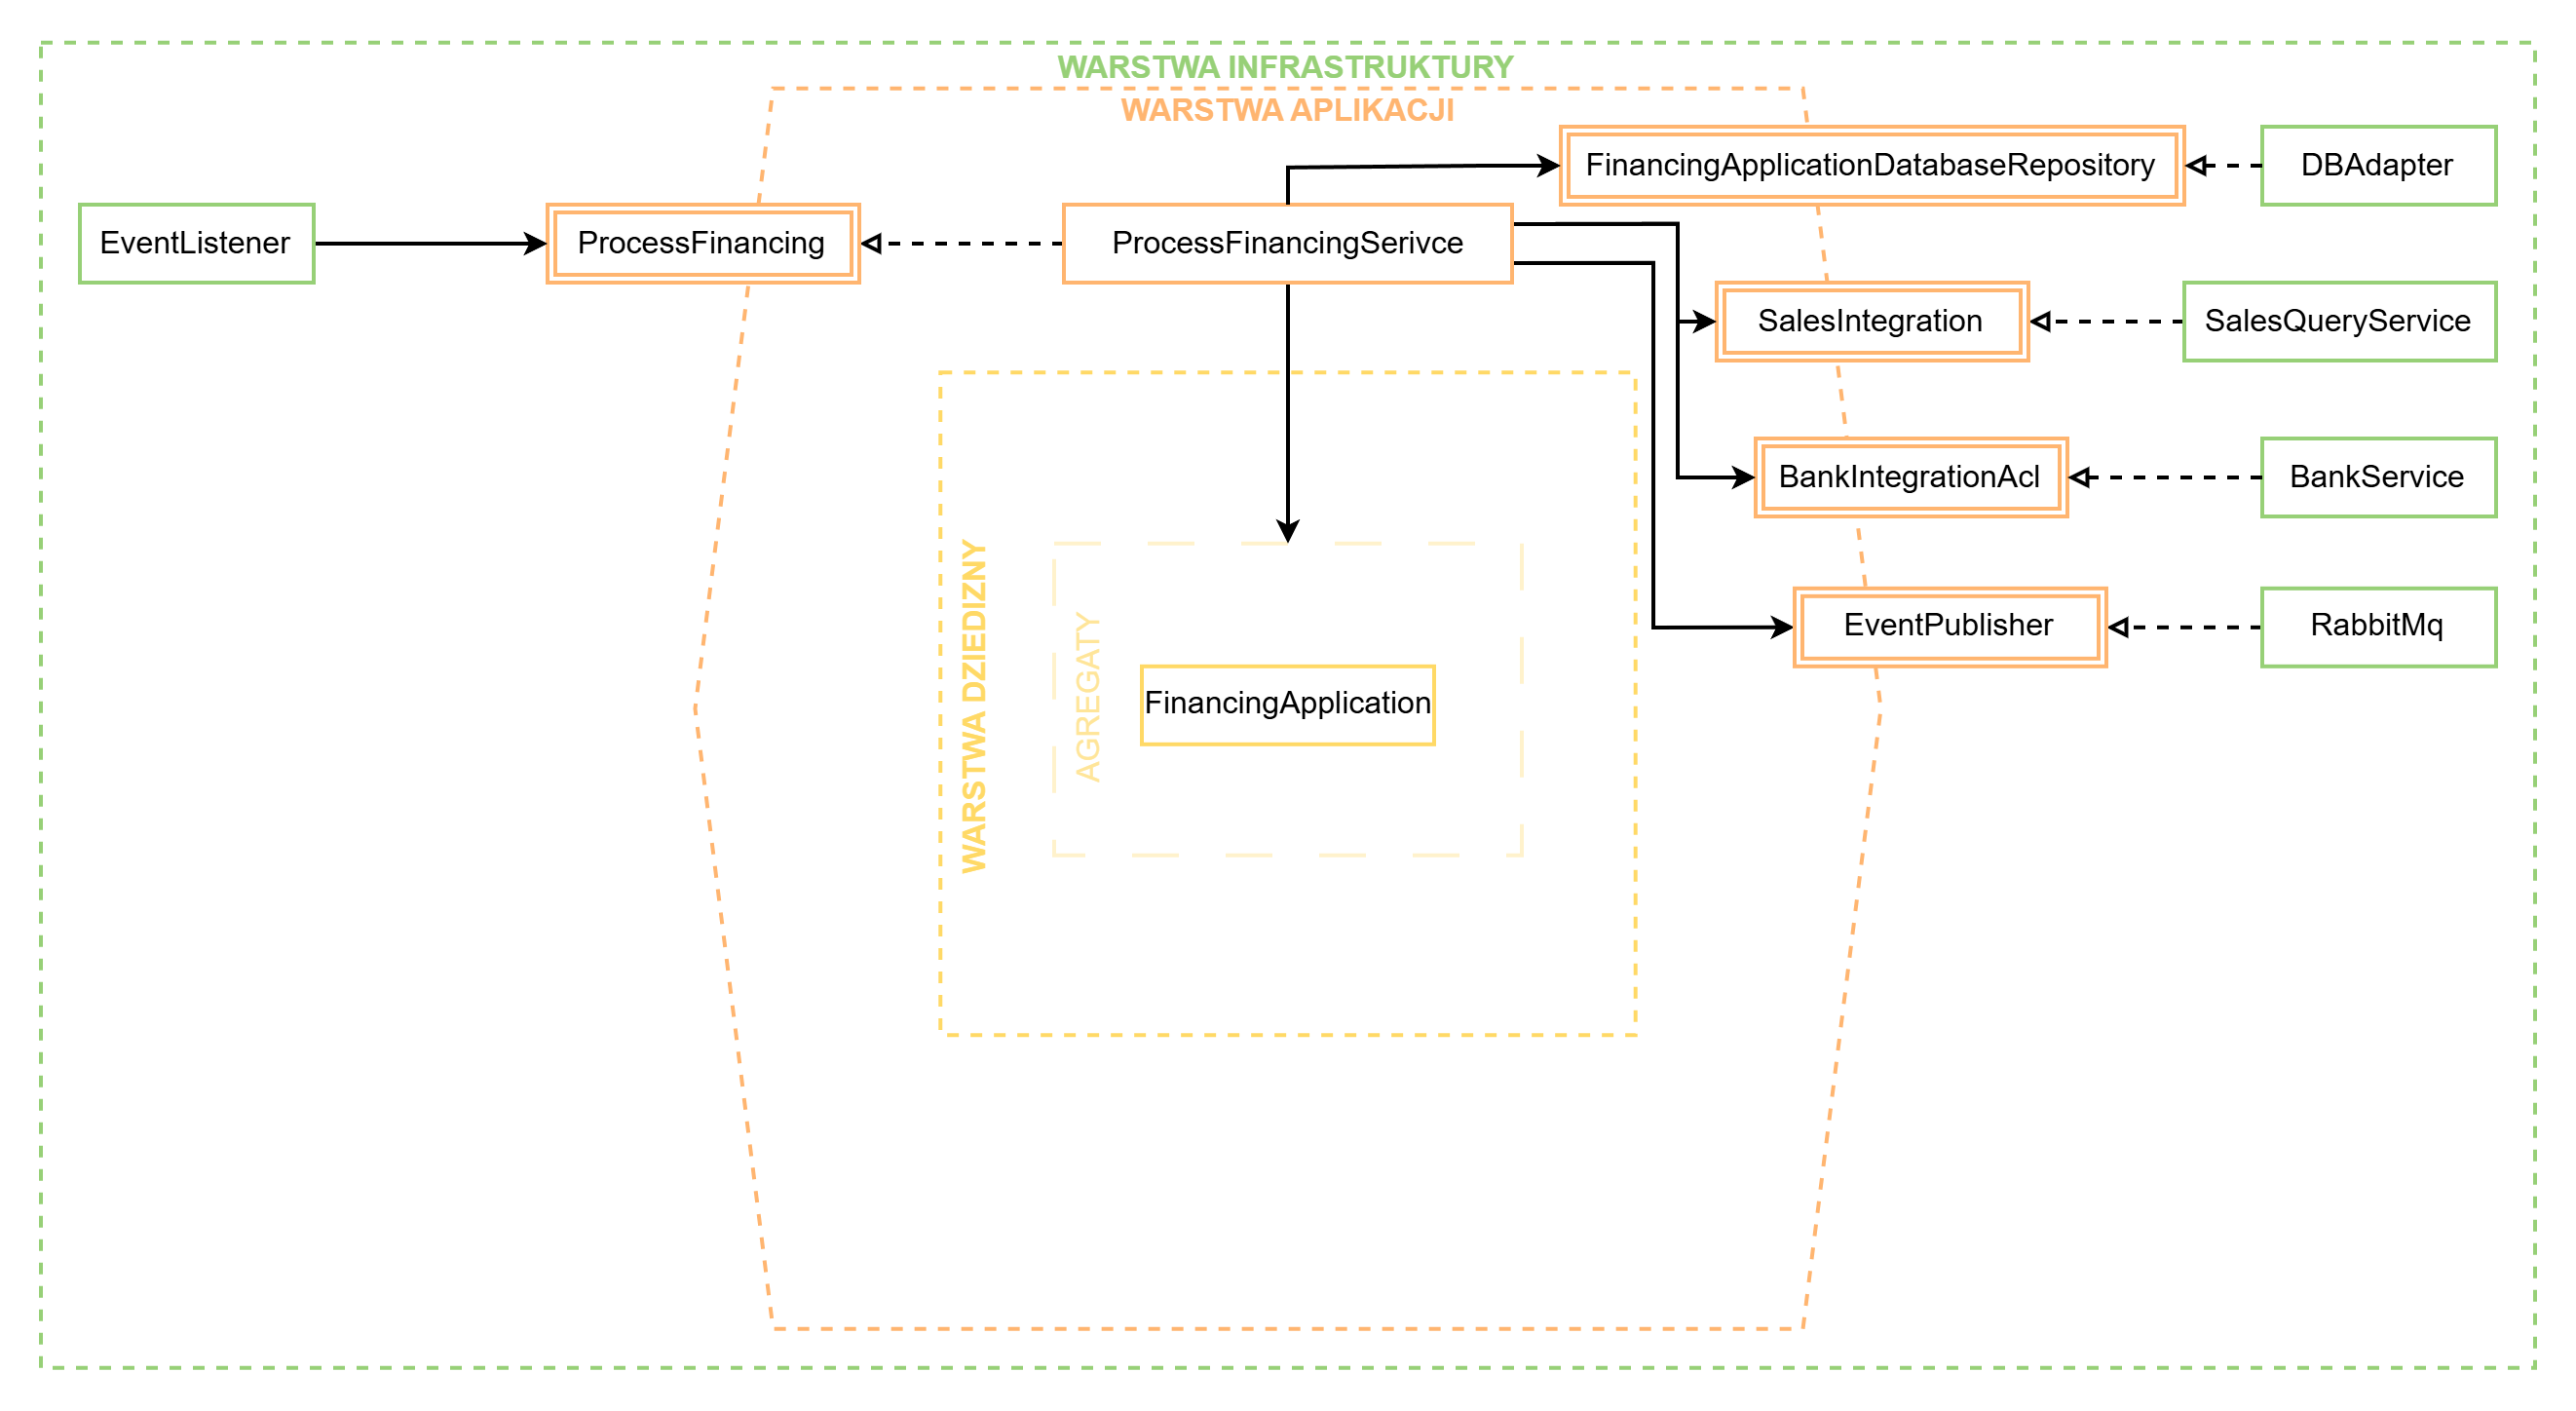
\includegraphics[width=\textwidth]{media/architektura_heksagonalna/FinancingArchitecture.png}
    \caption{Architektura heksagonalna kontekstu finansowania}
    \label{fig:hex_finance}
\end{figure}

Poniżej przedstawiono szczegółowy opis interakcji pomiędzy warstwami, z podziałem na strony wejściową i wyjściową.

\paragraph{Strona Wejściowa: Porty i Adaptery} 
Ta strona heksagonu definiuje, w jaki sposób świat zewnętrzny komunikuje się z Kontekstem Finansowania w celu wyzwolenia procesów oceny zdolności i akceptacji wniosków. Interfejsy wejściowe zestawiono z ich technicznymi implementacjami.

Zgodnie z diagramem Kontekst Finansowania udostępnia \textbf{jeden} port wejściowy obejmujący oba przypadki użycia (złożenie wniosku i przetworzenie decyzji banku), zasilany asynchronicznie zdarzeniami.

\begin{itemize}
    \item \textbf{Obsługa Wniosku o Finansowanie (Asynchroniczne)}
    \begin{itemize}
        \item \textbf{Port:} \texttt{ProcessFinancing}. Jedyny port wejściowy, obejmujący złożenie wniosku (\texttt{requestFinancing}, UC-FIN-01) oraz przetworzenie asynchronicznej decyzji banku (\texttt{processBankDecision}, UC-FIN-02). Realizowany przez usługę aplikacyjną \texttt{ProcessFinancingService}. Salon nie podejmuje decyzji kredytowej — bank jest jedynym decydentem, a port jedynie odzwierciedla nadany przez niego status.
        \item \textbf{Adapter:} \texttt{FinancingEventListener} (Messaging Adapter). Nasłuchuje magistrali zdarzeń: przechwytuje \texttt{FinancingRequested} (z Kontekstu Sprzedaży) i wyzwala \texttt{requestFinancing}, oraz \texttt{FinancingDecisionReceivedFromBank} (z adaptera bankowego) i wyzwala \texttt{processBankDecision}. Komunikaty zewnętrzne reprezentowane są jako lokalne rekordy ACL.
    \end{itemize}
\end{itemize}

\paragraph{Strona Wyjściowa: Porty i Adaptery} 
Ta strona heksagonu definiuje mechanizmy integracji warstwy aplikacji z bazą danych, zewnętrznymi instytucjami weryfikacyjnymi oraz systemem komunikacji asynchronicznej.

\begin{itemize}
    \item \textbf{Utrwalanie Stanu (Persystencja)}
    \begin{itemize}
        \item \textbf{Port:} \texttt{FinancingApplicationDatabaseRepository}. Umożliwia usłudze aplikacyjnej zapis i odczyt agregatu \texttt{FinancingApplication} (indeks po \texttt{OrderId}).
        \item \textbf{Adapter:} \texttt{InMemoryFinancingRepository} (węzeł \texttt{DBAdapter}). W bieżącej implementacji atrapa w pamięci; docelowo adapter bazodanowy (ORM/Hibernate) bez zmiany kontraktu portu.
    \end{itemize}

    \item \textbf{Integracja z Bankiem (Anti-Corruption Layer)}
    \begin{itemize}
        \item \textbf{Port:} \texttt{BankIntegrationAcl}. Dwukierunkowy port wyjściowy do systemu banku — wysyłka wniosku (\texttt{submitFinancingApplication}); bank jest jedynym decydentem, a decyzja wraca później osobnym zdarzeniem.
        \item \textbf{Adapter:} \texttt{BankIntegrationMockAdapter}. Atrapa symulująca asynchroniczne złożenie wniosku; docelowo adapter HTTP do zewnętrznych dostawców usług finansowych, tłumaczący ich API na model domeny (ACL).
    \end{itemize}

    \item \textbf{Integracja ze Sprzedażą i CRM (Anti-Corruption Layer)}
    \begin{itemize}
        \item \textbf{Port:} \texttt{SalesIntegration}. Query Port dociągający dane nabywcy (\texttt{buyerDetails}) oraz cenę końcową oferty (\texttt{offerFinalPrice}) potrzebne do wniosku (UC-FIN-01).
        \item \textbf{Adapter:} \texttt{SalesCrmIntegrationAdapter}. Zależy wyłącznie od fasady Sprzedaży (\texttt{SalesQueryFacade}) i tłumaczy migawki na lokalny model Finansowania (\texttt{BuyerDetails}, \texttt{Money}).
    \end{itemize}

    \item \textbf{Publikacja Zdarzeń}
    \begin{itemize}
        \item \textbf{Port:} \texttt{EventPublisher} (port Wspólnego Jądra). Umożliwia publikację zdarzeń wynikowych na magistralę.
        \item \textbf{Adapter:} \texttt{RabbitMqEventPublisherAdapter} (Wspólne Jądro). Serializuje zdarzenia dziedzinowe o statusie wniosku (np. \texttt{FinancingApprovedEvent}, \texttt{FinancingRejectedEvent}, \texttt{FinancingApplicationFailedEvent}) i wysyła je na magistralę, umożliwiając modułowi Sprzedaży asynchroniczną kontynuację obsługi klienta.
    \end{itemize}
\end{itemize}

\paragraph{Usługi Aplikacji}
Dla kontekstu Finansowania przewidziano jeden centralny komponent orkiestrujący:
\begin{itemize}
    \item \textbf{ProcessFinancingService} – zarządza pełnym cyklem życia wniosku o finansowanie. W ramach UC-FIN-01 dociąga dane nabywcy i kwotę z Kontekstu Sprzedaży (\texttt{SalesIntegration}), tworzy nowy agregat \texttt{FinancingApplication} przez fabrykę (\texttt{createDraft}), wysyła wniosek do banku (\texttt{BankIntegrationAcl}) i utrwala status PENDING. W ramach UC-FIN-02 pobiera wniosek po \texttt{OrderId}, wymusza na nim mutację stanu zgodnie z decyzją banku (\texttt{approve}/\texttt{reject}) i emituje zdarzenia kończące proces.
\end{itemize}

\subsubsection{Agregaty Kontekstu Finansowania}

% MIEJSCE NA DIAGRAM KLAS: FinancingApplication
\begin{figure}[H]
    \centering
    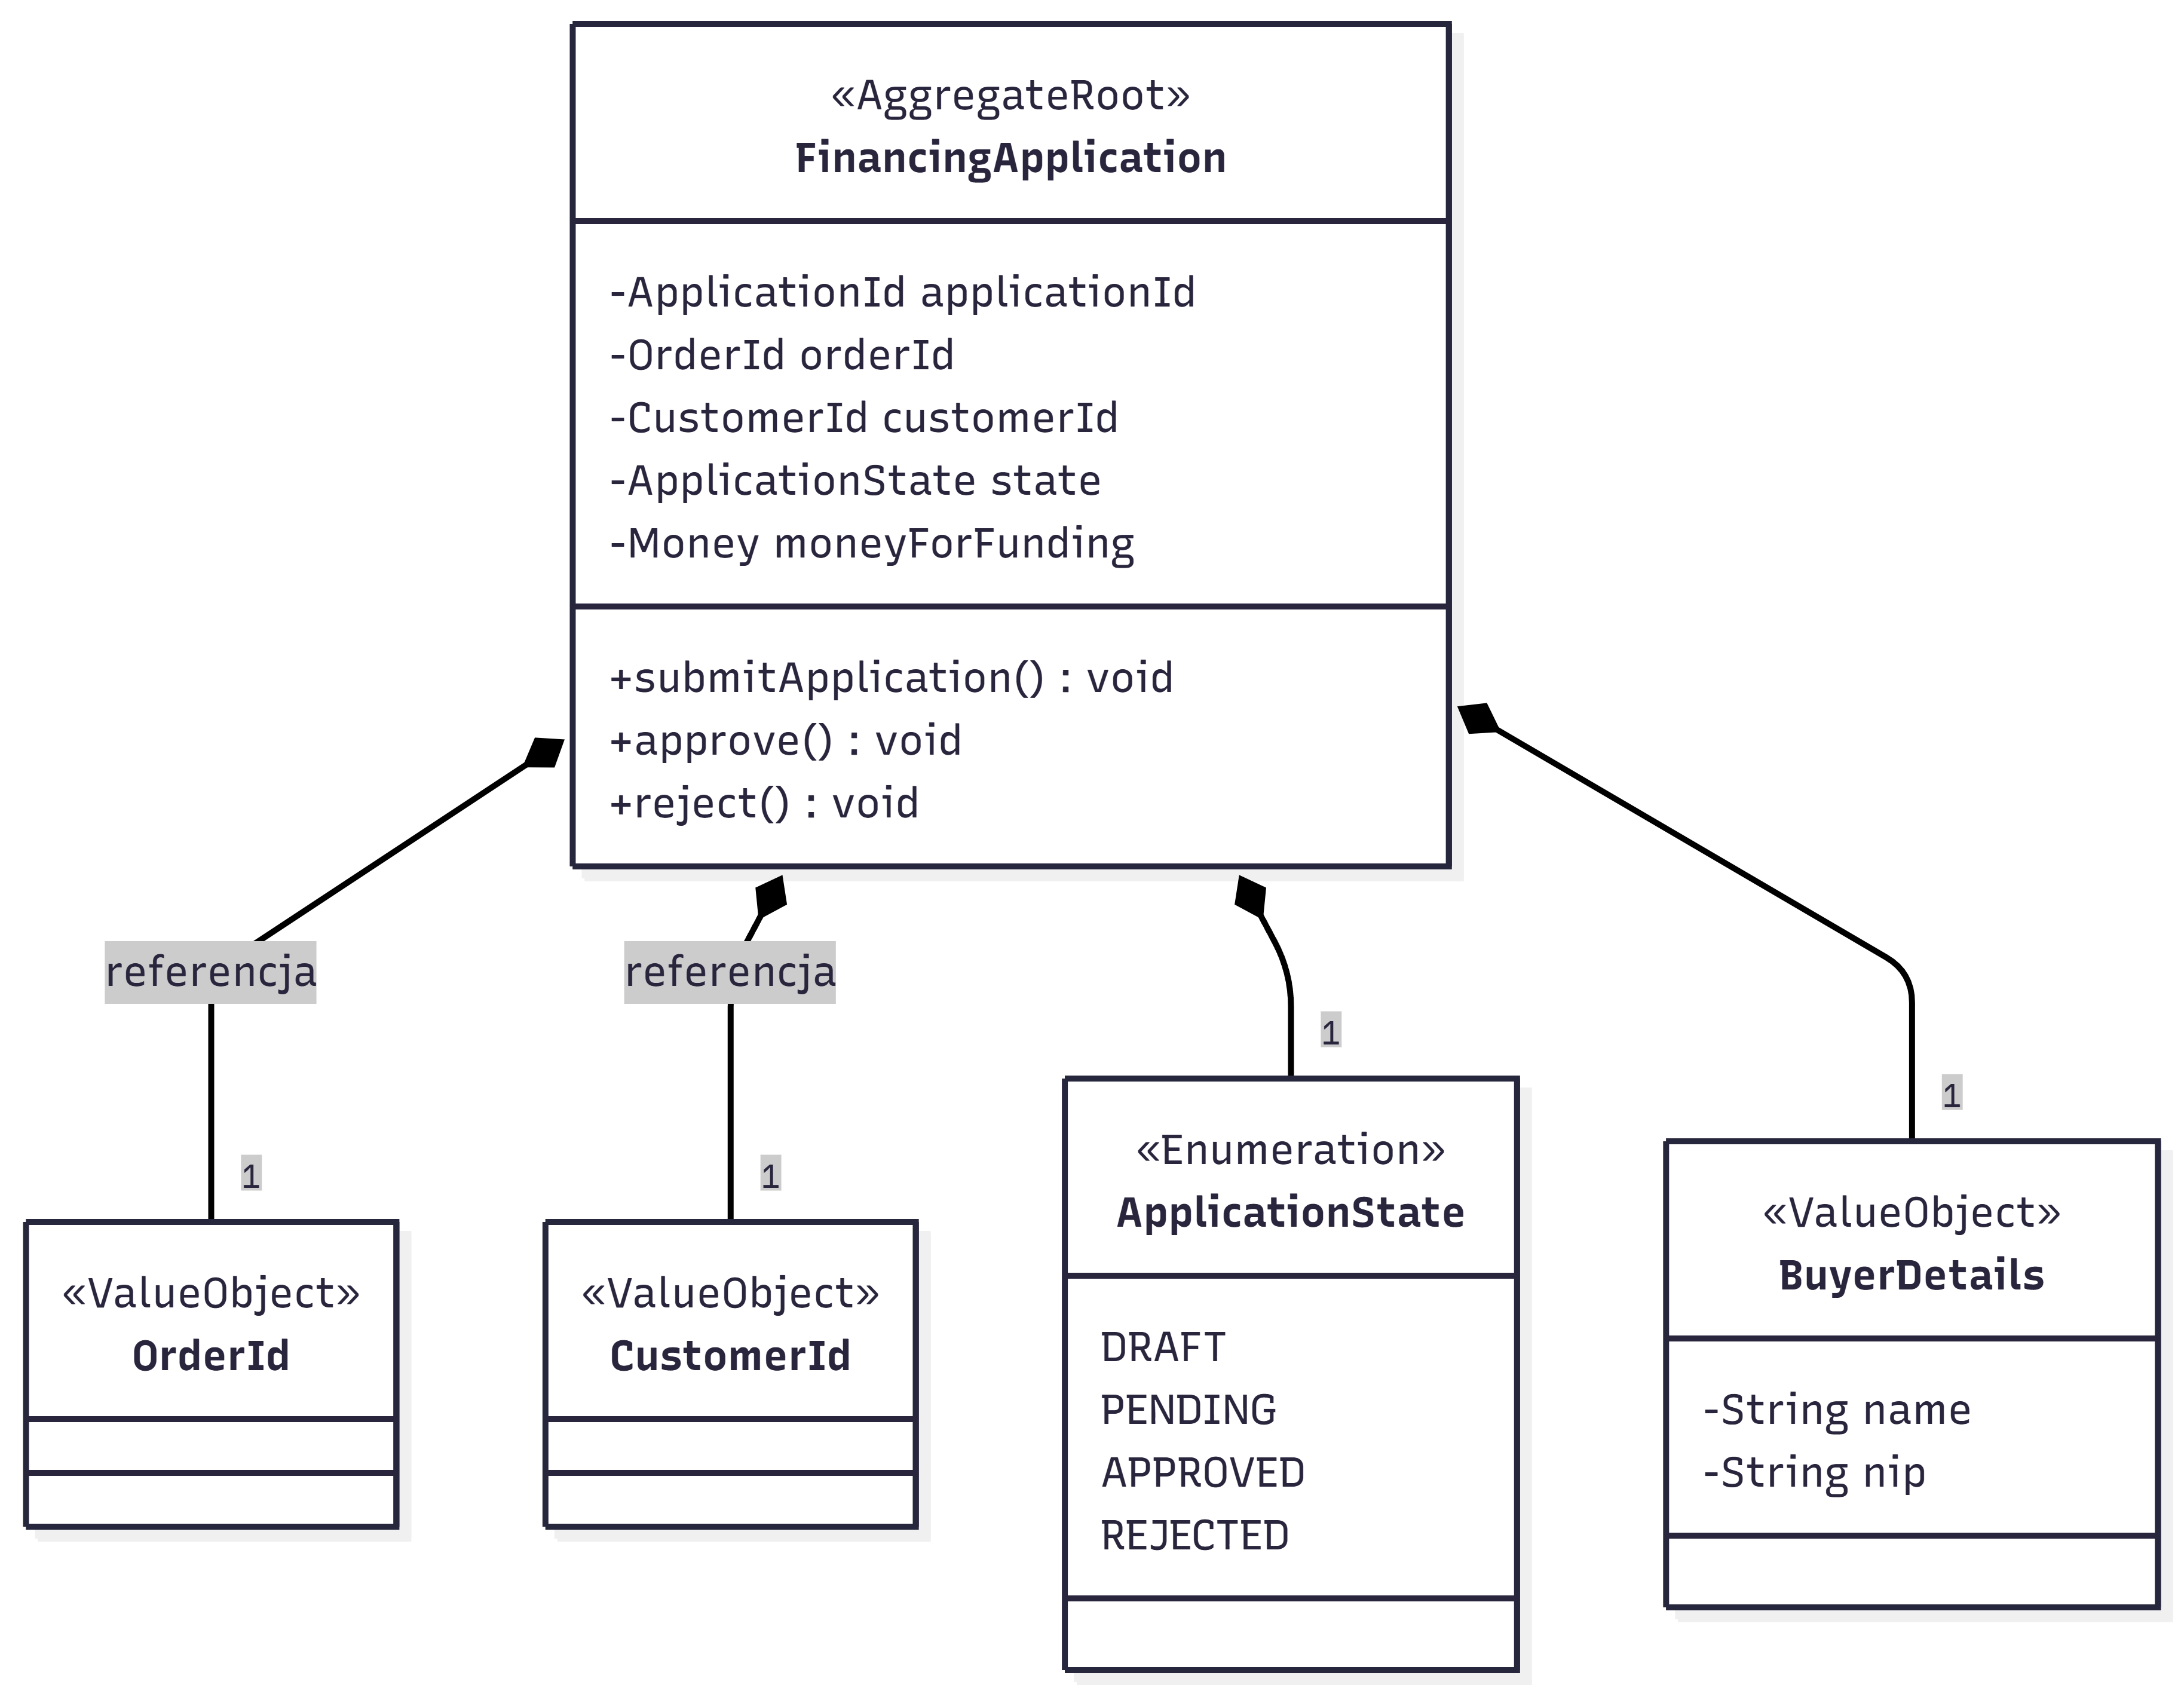
\includegraphics[width=0.5\textwidth]{media/agregaty/kontekst-finansowania/financing-application.png}
    \caption{Model strukturalny agregatu Wniosku Finansowego}
    \label{fig:agg_financing}
\end{figure}

Z uwagi na generyczny i integracyjny charakter tej poddziedziny, zrezygnowano ze skomplikowanych agregatów obliczeniowych na rzecz hermetycznych maszyn stanów.

\paragraph{Agregat: Wniosek Finansowy (FinancingApplication)}
Odpowiada za reprezentację procesu wnioskowania o leasing lub kredyt, powiązanego z danym Zamówieniem. Agregat został maksymalnie zdenormalizowany - nie przechowuje szczegółowych danych finansowych czy analitycznych, skupiając się wyłącznie na bezpiecznym śledzeniu cyklu życia procesu integracyjnego.
\begin{itemize}
    \item \textbf{Maszyna Stanów:} Agregat operuje na ściśle zdefiniowanych stanach (np. \texttt{DRAFT}, \texttt{PENDING}, \texttt{APPROVED}). Zmiana stanu wymuszana jest poprzez hermetyczne metody (\linebreak \texttt{submitApplication}, \texttt{approve}, \texttt{reject}).
    \item \textbf{Ochrona Niezmienników:} Wysłanie wniosku do banku zmienia jego stan na \texttt{PENDING}. Agregat kategorycznie zabrania wywołania metody \texttt{approve()} z jakiegokolwiek innego stanu. Jeśli zewnętrzne API banku w wyniku błędu prześle podwójny webhook z potwierdzeniem finansowania, agregat odrzuci drugą próbę, chroniąc system przed wyemitowaniem zduplikowanych zdarzeń dziedzinowych i podwójnym finansowaniem zamówienia.
    \item \textbf{Sterowanie Przepływem Systemu:} Dopiero pomyślne zatwierdzenie wniosku i zmiana stanu na \texttt{APPROVED} powoduje wewnątrz agregatu wygenerowanie krytycznego zdarzenia \linebreak \texttt{FinancingApprovedEvent}, na które nasłuchuje m.in. Kontekst Rozliczeń, w celu weryfikacji ostatecznego salda kontraktu.
\end{itemize}